%
% normalenform.tex
%
% (c) 2018 Prof Dr Andreas Müller, Hochschule Rapperswil
%
\documentclass[tikz]{standalone}
\usepackage{times}
\usepackage{amsmath}
\usepackage{txfonts}
\usepackage{ifthen}
\usepackage[utf8]{inputenc}
\usepackage{graphics}
\usetikzlibrary{arrows,intersections,math}
\begin{document}
\newboolean{gitter}
\setboolean{gitter}{false}

\begin{tikzpicture}[>=latex,thick]

\node at (0,0) {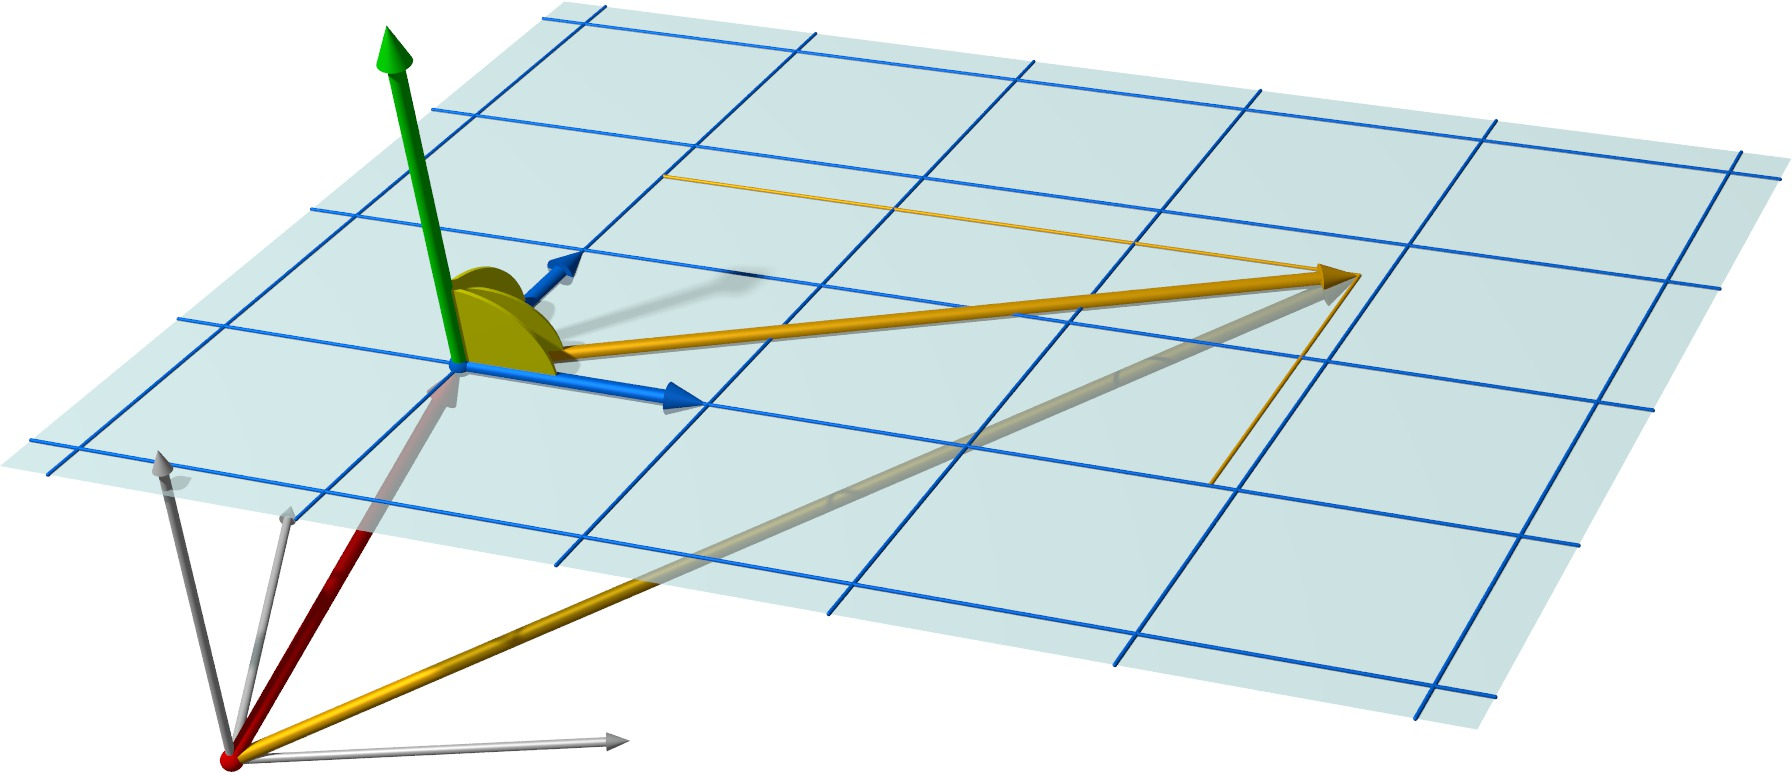
\includegraphics[width=16cm]{normalenform.jpg}};

\ifthenelse{\boolean{gitter}}{
\foreach \x in {-8,-7,...,8}{
	\draw[line width=0.1pt] (\x,-4)--(\x,4);
}
\foreach \y in {-4,-3,...,4}{
	\draw[line width=0.1pt] (-8,\y)--(8,\y);
}
\fill (0,0) circle[radius=1pt];
}{}

\node at (-1.65,-0.4) {$\vec{u}$};
\node at (-2.8,1.45) {$\vec{v}$};
\node at (-4.8,3.3) {$\vec{n}$};

\node at (-4.25,0.05) {$P$};
\node at (-4.7,-1.8) {$\vec{p}$};

\node at (4.2,1.2) {$Q$};
\node at (-2.7,-2.3) {$\vec{q}$};

\node at (1.2,1.0) {$\vec{q}-\vec{p}$};

\node at (-6.2,-3.4) {$O$};

\end{tikzpicture}

\end{document}

